\chapter{\textit{\textbf{Elastic stack}}}
U ovom poglavlju biće opisan \textit{\textbf{Elastic stack}}, kao primer alata za obradu velikih skupova podataka u realnom vremenu. Bitno je napomenuti da se dalji tekst oslanja na dokumentaciju trenutno najnovije javno dostupne verzije alata 8.6 \cite{elastic-stack-docs}, odnosno najnovije verzije komponenti koje čine alat, a koje će biti istaknute pri obrađivanju svake od komponenti. U ovom poglavlju će, između ostalog, biti opisani delovi alata neophodni za implementaciju sistema koja će biti data u sledećem poglavlju kao primer korišćenja alata.

\section{Osnove \textit{\textbf{Elastic stack}}-a}
\textit{\textbf{Elastic stack}}, takođe poznat kao \textit{\textbf{ELK stack}}, predstavlja alat, koji postoji kao otvoreno rešenje \textit{(eng. open source)} kompanije \textit{\textbf{Elastic}} \cite{elastic-site}, a čije funkcionalnosti podrazumevaju: prikupljanje podataka u bilo kom formatu, njihovu obradu, nadogradnju, skladištenje, pretraživanje, analizu i vizuelizaciju u realnom vremenu. Akronim \textit{ELK} identifikuje ključne komponente ovog steka, a to su: \textit{\textbf{Elasticsearch}} \cite{elastic-elasticsearch}, \textit{\textbf{Logstash}} \cite{elastic-logstash} i \textit{\textbf{Kibana}} \cite{elastic-kibana}.

\par
Apstrakcija toka podataka je prikazana na slici \ref{diagram:apstrakcija-toka-podataka-kroz-ELK-stack}. Podaci mogu doći iz bilo kog izvora, što je na slici generalizovano komponentom \textit{Beats} \cite{elastic-beats}, koja predstavlja opcioni dodatak \textit{\textbf{ELK stack}}-a i služi za slanje operativnih podataka na \textit{\textbf{Logstash}}. \textit{\textbf{Logstash}} komponenta predstavlja uređivač \textit{(eng. formatter)} sistema, njena glavna funkcionalnost jeste prikupljanje ulaznih podataka bilo kog formata, parsiranje podataka i slanje istih u željenom obliku na \textit{\textbf{Elasticsearch}}. \textit{\textbf{Elasticsearch}} uz pomoć indeksa vrši skladištenje podataka i olakšava njihovo pretraživanje, takozvano pretraživanje celog teksta \textit{(eng. full-text search)}. Tako indeksirani podaci se uz pomoć \textit{\textbf{Kibana}} mogu vizualno prikazivati i ujedno se vršiti njihova analiza.
Neke od najčešćih vrsta podataka koji se obrađuju uz pomoć \textit{\textbf{ELK stack}}-a podrazumevaju: evidentirane \textit{(eng. logged)}, metričke, bezbednosne i podatke biznis logike.

\begin{figure}[H]
    \centering
    \fboxsep=0.025\columnwidth%padding thickness
    \fboxrule=1pt%border thickness
    \fbox{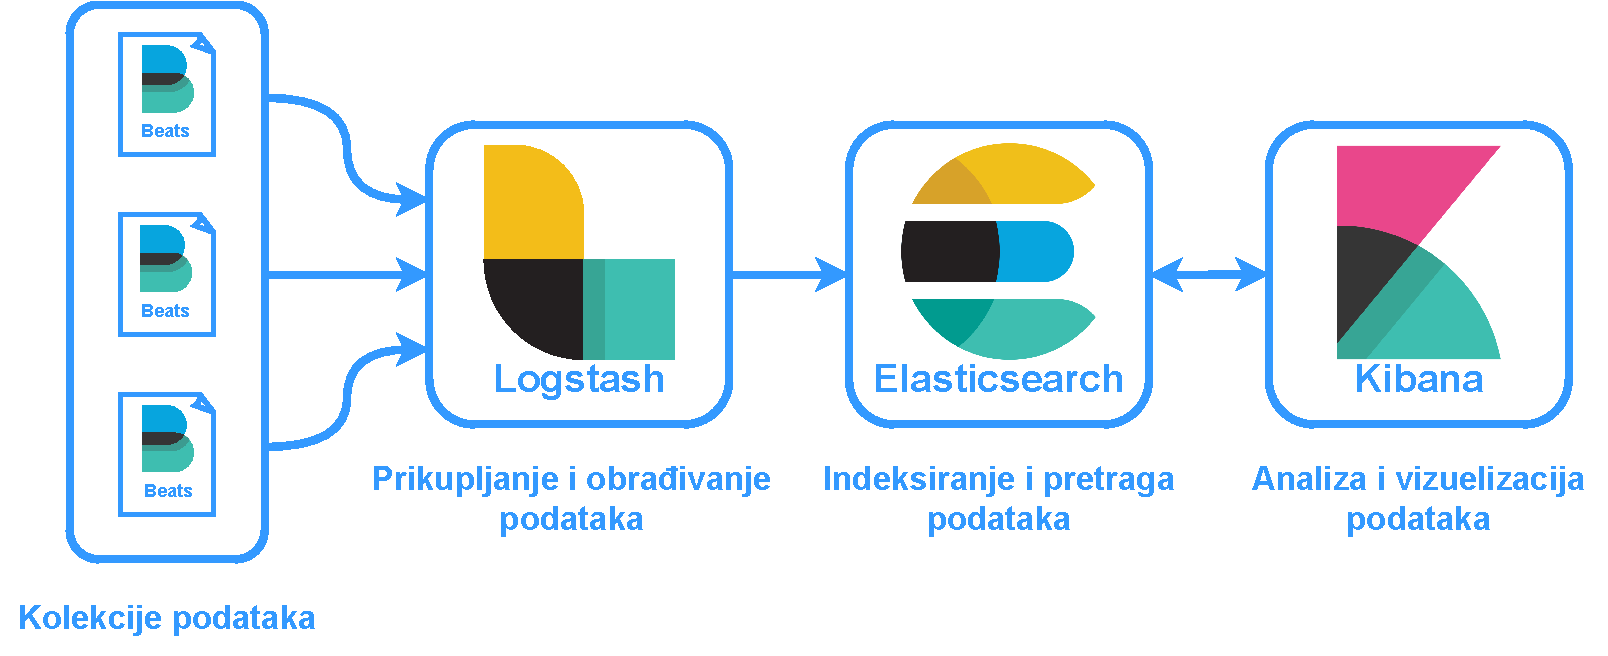
\includegraphics[width=0.95\columnwidth]{images/ELK stek.pdf}}
    \caption{\textit{Apstrakcija toka podataka kroz \textbf{ELK stack}}}
    \label{diagram:apstrakcija-toka-podataka-kroz-ELK-stack}
\end{figure}

\section{\textit{\textbf{Elasticsearch}}}
\textit{\textbf{Elasticsearch}} je besplatan, distribuirani, otvoreni alat za skladištenje, pretragu i analizu \textit{(eng. search and analytics engine)}, raznih tipova podataka, uključujući tekstualne, numeričke, geo-prostorne \textit{(eng. geospatial)}, strukturne i nestrukturne \cite{elastic-elasticsearch}. Manipulacija podataka je ostvarena \textit{REST API}-jem, a alat omogućava izvanrednu horizontalnu skalabilnost. \textit{\textbf{Elasticsearch}} je zasnovan na \textbf{\textit{Apache Lucene} biblioteci} \cite{apache-lucene}, tj. ideji indeksiranja podataka na osnovu samog sadržaja. Podaci se skladište kao dokumenti, koji pripadaju jednom indeksu, dok je uz pomoć distribuiranog modela, indekse moguće podeliti na manje komponente, odnosno krhotine \textit{(eng. shard)}, koji mogu biti rasprostranjeni kroz veći broj čvorova \textit{(eng. node)}. Trenutno aktuelna verzija na kojoj se zasniva opis alata jeste verzija 8.6.

\subsection{Osnove \textit{\textbf{Elasticsearch}}-a}\label{subsection:osnove-elasticsearch-a}
\textit{\textbf{Elasticsearch}} arhitektura je projektovana za prikupljanje dokumenata, koji se skladište kao \textit{JSON} objekti \cite{json}. Alat podržava ugnježdene strukture, što olakšava obradu kompleksnih podataka i upita. Za praćenje informacija o dokumentima dodeljuju se specijalni atributi, odnosno meta-podaci, koji počinju donjom crtom. Važni meta-podaci su:
\begin{itemize}
    \item \textbf{\_index} – predstavlja kom indeksu dokument pripada. U analogiji, npr. sa relacionim bazama, ovo bi predstavljalo jednu bazu podataka.
    \item \textbf{\_type} – predstavlja klasu, odnosno mapiranje koje bi trebalo da ima svaki dokument koji pripada istom tipu. Ovo je analogno tabeli u relacionim bazama podataka. Trenutna verzija alata ovo polje tretira kao zastarelo \textit{(eng. deprecated)}, ostavljeno je samo radi kompatibilnosti sa starijim verzijama alata.
    \item \textbf{\_id} – jedinstveni identifikator dokumenta u okviru tipa.
    \item \textbf{\_version} – predstavlja broj izmena dokumenta, odnosno koliko puta je dokument bio kreiran, ažuriran, obrisan.
\end{itemize}

\par
Glavni elementi arhitekture \textit{\textbf{Elasticseach}}-a su: \textbf{klaster}, \textbf{čvor}, \textbf{krhotina} i \textbf{analizator}, čija je organizacija predstavljena na slici \ref{diagram:ahritektura-elasticsearch-alata}.

\begin{figure}[H]
    \centering
    \fboxsep=0.025\columnwidth%padding thickness
    \fboxrule=1pt%border thickness
    \fbox{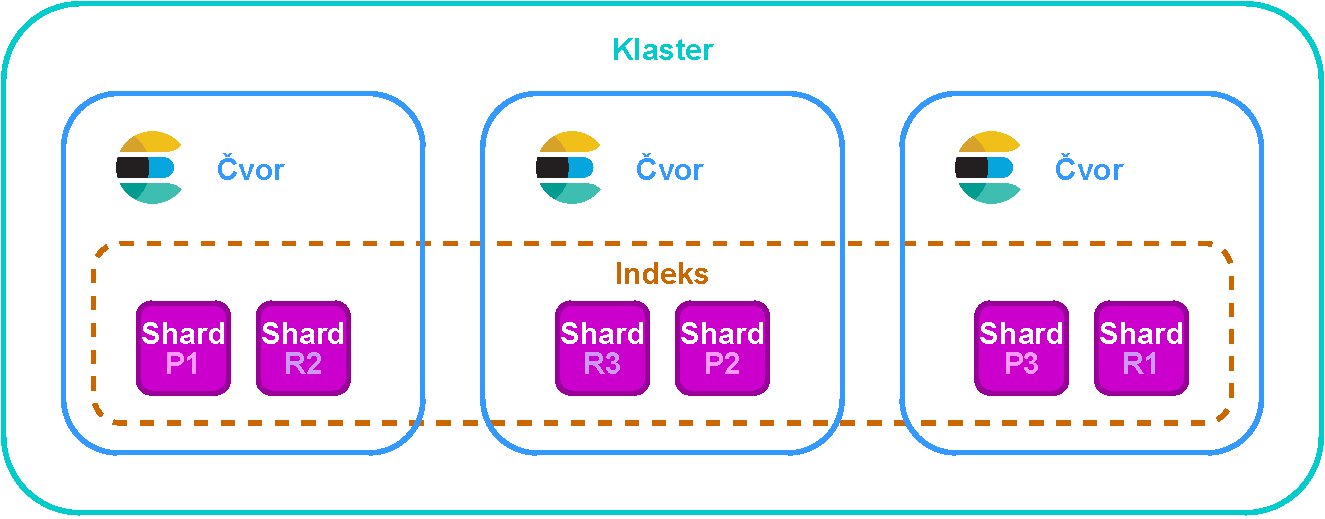
\includegraphics[width=0.95\columnwidth]{images/Elasticsearch-architecture.pdf}}
    \caption{\textit{Arhitektura \textbf{Elasticsearch} alata}}
    \label{diagram:ahritektura-elasticsearch-alata}
\end{figure}

\par
\textbf{Klaster} predstavlja grupu čvorova koji skladište podatke. U okviru konfiguracionog fajla \textit{\textbf{config/Elasticsearch.yml}} \footnote{\textit{YAML} format je dostupan u okviru \cite{YAML}} se može precizirati broj čvorova koji bivaju startovani u klasteru, kao i fizička ili virtualna adresa svakog od čvorova. Čvorovi u okviru jednog klastera su logički povezani i mogu razmenjivati podatke jedni sa drugima. Pri pokretanju, sistem automatski kreira jedan klaster sa jednim čvorom u njemu, što je dovoljno za osnovne potrebe prosečnog korisnika.

\par
\textbf{Čvor} ne predstavlja server, već jednu instancu \textit{\textbf{Elasticsearch}}-a, odnosno proces. Svaka instanca pripada jednom klasteru i zajedno, sa ostalim čvorovima u klasteru radi na rešavanju istog zadatka. Svaki čvor se može konfigurisati tako da obavlja barem jednu, a može obavljati više uloga u klasteru. Uloge koje čvoru mogu biti dodeljene obuhvataju:
\begin{itemize}
\item \textbf{Master čvor} – vrši kontrolu nad klasterom u vidu koordinacije čvorova koji pripadaju klasteru. Ovi čvorovi su odgovorni za operacije nad klasterom \textit{(eng. clasterwide operations)}, poput kreiranja i brisanja indeksa.
\item \textbf{Data čvor} – vrši skladištenje i odgovoran je za invertovani indeks podataka. Ovo je podrazumevana uloga čvora.
\item \textbf{Klijentski čvor} – predstavlja raspoređivač opterećenja \textit{(eng. load balancer)}\cite{Sanders2019-hv} koji vrši usmeravanje pristiglih zahteva različitim čvorovima u klasteru.
\end{itemize}

\par
Za ostvarivanje komunikacije se koriste dva glavna porta:
\begin{itemize}
    \item \textbf{Port 9200} – koristi se za filtriranje zahteva koji dolaze izvan klastera. Ovo su zahtevi \textit{REST API}-ja koji se koriste za izvršavanje upita, indeksiranje i slično.
    \item \textbf{Port 9300} – koristi se za među-čvornu \textit{(eng. inter-node)} komunikaciju.
\end{itemize}

\par
\textbf{Krhotina} predstavlja podskup dokumenata u okviru jednog indeksa. Naime, indeks nema ograničen broj dokumenata, niti ograničen memorijski kapacitet koji može da skladišti. Ukoliko se desi prekoračenje memorije na jednom od čvorova, \textit{\textbf{Elasticsearch}} prestaje sa radom i javlja grešku. Kako bi se ovaj problem rešio, indeksi se dele na krhotine, koje označavaju skalabilnu jedinicu za indeksiranje i omogućavaju distribuciju jednog indeksa na više čvorova. Ovim se postiže horizontalna skalabilnost sistema. Svaka krhotina funkcioniše kao nezavisan \textit{Lucene} indeks \cite{apache-lucene}, koji može biti skladišten bilo gde u klasteru.

\par
\textbf{Replika} predstavlja kopiju krhotine indeksa, dok se originalna krhotina naziva primarnom \textit{(eng. primary shard)}. Redundantnost podataka je glavni mehanizam na koji se sistemi otporni na greške oslanjaju \cite{Sanders2019-hv}. S obzirom da se radi o distribuiranom sistemom, ukoliko bi neki od čvorova otkazao, krhotine indeksa koje sadrži bi bile nedostupne, a samim tim i svi dokumenti koji se nalaze u nedostupnim podskupovima. Iz tog razloga se formiraju replike i dodeljuju različitim čvorovima u sistemu. Pored otpornosti na otkaze, ovo omogućava i brže pretraživanje podataka, jer više čvorova koji sadrže istu kopiju krhotine indeksa mogu istovremeno da vrše njenu pretragu i time ubrzaju proces pretrage indeksa u celini. Broj replika nije ograničen i mogu se precizirati nakon kreiranja indeksa, međutim, treba voditi računa jer iako je ovim čitanje ubrzano, svaka modifikacija je time znatno složenija.

\par
\textbf{Analizatori} imaju zadatak da vrše parsiranje fraza i izraza u konzistentne termine. Ovo se odvija u procesu indeksiranja. Svaki analizator je sačinjen od jednog tokenizatora \textit{(eng. tokenizer)} \footnote{Tokenizacija je proces razgraničenja i moguće klasifikacije delova niza ulaznih znakova. Dobijeni tokeni se zatim prosleđuju nekom drugom obliku obrade. Proces se može smatrati podzadatkom raščlanjivanja ulaza.\cite{tokenization}} i većeg broja filtera tokena. Kada se naiđe na određeni izraz, tokenizator može da podeli izraz u prethodno definisane termine. U ovome se krije još jedna tajna brze pretrage podataka.

\input{poglavlja/telo/01-elastic-stack/02-Logstash.tex}
\section{\textit{\textbf{Kibana}}}
\textit{\textbf{Kibana}} je aplikacija otvorenog koda koja pruža pregledan korisnički interfejs ka \textit{Elastic stack}-u, uz mogućnosti pretraživanja, vizuelizacije i analize podataka indeksiranih \textit{Elasticsearch}-om. Takođe poznata i kao alat za kreiranje raznovrsnih grafikona \textit{(eng. charts)}, \textit{\textbf{Kibana}} omogućava nadgledanje, upravljanje i održavanje bezbednosti klastera u \textit{Elastic stack}-u. Prvi put je postala dostupna javnosti 2013. godine, dok je trenutna aktuelna verzija 8.6, na osnovu koje će biti opisani pojedini detalji same aplikacije \cite{elastic-kibana}.

\par
Glavna primena \textit{\textbf{Kibana}}-e podrazumeva: pretraživanje, vizualizaciju indeksiranih podataka u okviru \textit{Elasticsearch}-a, kao i analizu podataka kroz kreiranje grafikona, poput: poluga, pita, tabela, histograma i mapa. Komandna tabla \textit{(eng. dashboard)} kombinuje ove elemente na jedan pano i time omogućava analitički pregled podataka u realnom vremenu za razne slučajeve korišćenja, poput:
\begin{enumerate}
    \item analize podataka evidencije, 
    \item nadgledanja metričkih podataka infrastrukture i kontejnera, 
    \item vizuelizaciju geo-prostornih podataka, 
    \item analizu sigurnosnih podataka, 
    \item analizu podataka biznis logike.
\end{enumerate}

\subsection{Upitni jezik \textit{\textbf{Kibana}}-e}
\textit{\textbf{Kibana}} koristi specifični upitni jezik nazvan \textit{\textbf{Kibana Query Language}} \cite{kql}, ili skraćeno \textit{\textbf{KQL}}, kojim je omogućeno jednostavno filtriranje podataka u svrhu vizualizacije. Ovaj jezik se razlikuje od standardnog \textit{Lucene }upitnog jezika, jer ne omogućava pretragu uz pomoć regularnih izraza ili takozvanu pomućenu \textit{(eng. fuzzy)} pretragu podataka, međutim omogućena je pretraga ugnježdenih polja kao i takozvanih skriptovanih polja \textit{(eng. scripted fields)}.

\par
U okviru jezika se mogu identifikovati podvrste upitnog jezika: \textbf{upiti termina}, \textbf{upiti Bulove algebre}, \textbf{opsežni upiti}, \textbf{upiti koji koriste džokere} i \textbf{upiti nad ugnježdenim poljima}.

\par
\textbf{Upiti termina} \textit{(eng. terms query)}, koji koriste egzaktan stil pretrage. Sintaksa ovog upita ima oblik \textit{<putanja do polja> : <list termina>}, gde putanja do polja predstavlja ugnježdena polja počevši od korena dokumenta, sve do polja koje se pretražuje, nivoi su razdvojeni tačkom. Lista termina predstavlja prihvatljive vrednosti u okviru navedenog polja, dok se različiti termini odvajaju razmakom, a ukoliko se pretražuju egzaktne fraze, koriste se znaci navođenja. Putanja do polja i lista termina se odvajaju specijalnim karakterom dvotačka, na koji može da se gleda kao na operator \textit{in}.

\par
\textbf{Upiti Bulove algebre} \textit{(eng. boolean queries)} predstavljaju kombinovanje prethodno navedene podvrste upita logičkim operatorima: \textbf{or}, \textbf{and} i \textbf{not}. Po pravilu, \textbf{and} ima viši prioritet od operatora \textbf{or}, ukoliko je neophodna drugačija logika, koriste se zagrade.

\par
\textbf{Opsežni upiti} \textit{(eng. range queries)} predstavljaju upite koji numeričke i vrednosti datuma navedenih polja porede operatorima jednakosti: \textbf{>}, \textbf{>=}, \textbf{<} i \textbf{<=}. Moguće je koristiti i matematičke izraze pri poređenju vrednosti, što je jako pogodno za datume.

\par
\textbf{Upiti koji koriste džokere} \textit{(eng. wildcard)}, koji je označen znakom \textbf{*} i može biti ili u delu putanje polja, čime se pokriva veći broj polja, ili u okviru vrednosti koje se traže u poljima i time pokriva veći spektar vrednosti, jer menja odgovarajući deo bilo kojom sekvencom bilo koje dužine.

\par
\textbf{Upiti nad ugnježdenim poljima} \textit{(eng. nested field queries)} omogućavaju dva pristupa u filtriranju ugnježdenih dokumenata:
\begin{itemize}
    \item Filtriranje jednog dokumenta na osnovu određenih delova upita\\
\textit{<polje>:\{ <ugnježdeno polje 1>:<izraz 1> and <ugnježdeno polje 2>:<izraz 2> \}}
    \item Filtriranje više dokumenata na osnovu određenih delova upita \\
\textit{<polje>:\{ <ugnježdeno polje 1>:<izraz 1> \} and <polje>:\{ <ugnježdeno polje 2>:<izraz 2> }\}
\end{itemize}